\subsection{向量子空间与正交投影算子}

设 \(\mathbf{E}\) 为准希尔伯特空间。回顾，两个向量 \(x\) 与 \(y\) （属于 \(\mathbf{E}\) ）称为正交的，如果 \(\langle x|y\rangle = 0\) ；这时

\[
\| x + y \| ^ {2} = \| x \| ^ {2} + \| y \| ^ {2}\tag{16}
\]

（«勾股定理»）。

设 A 为 E 的子集。我们说 E 中的向量 x 与 A 正交，如果它与 A 的每个向量正交。与 A 正交的全体向量组成的集是 A 的一个闭向量子空间，记作 \(A^{\circ}\) ，（滥用术语）称为 A 的正交。

设 A 与 B 为 E 的两个子集。我们说 A 与 B 正交，如果 A 的每个向量与 B 的每个向量正交。这等价于说 \(A \subset B^{\circ}\) ，或 \(B \subset A^{\circ}\) 。若 E 是 Hausdorff 的且 A 与 B 正交，则 \(A \cap B\) 为空或化为 0，因为 0 是 E 中与自身正交的唯一向量。

定理 2. --- 设 E 为准希尔伯特空间，M 为 E 的一个向量子空间，且它是 Hausdorff 的和完备的。则 E 是 M 与 \(M^{\circ}\) （与 M 正交的子空间）的拓扑直和。与分解 \(E = M \oplus M^{\circ}\) 相伴的从 E 到 M 上的投影算子是定理 1（V, p.~10）中定义的从 E 到 M 上的投影 \(p_{M}\) 。

我们首先证明 \(x - p_{\mathbf{M}}(x)\) 属于 \(M^{\circ}\) 对所有 \(x \in E\) 成立。设 \(y \in M\) 。对每个标量 \(\lambda \in K\) ，向量 \(p_{\mathbf{M}}(x) + \lambda y\) 属于 M；于是由公式 15（V, p.~10）我们有，

\[
\mathcal {R} \big (\lambda \langle x - p _ {\mathrm{M}} (x) | y \rangle \big) \leqslant 0
\]

对所有 \(\lambda \in \mathbf{K}\) 成立。特别地，若取 \(\lambda = \overline{\langle x - p_{\mathbf{M}}(x)|y\rangle}\) ，便得出 \(\langle x - p_{\mathbf{M}}(x)|y\rangle = 0\) ，从而得到我们的断言。

由于 M 是 Hausdorff 的，0 是 M 中与自身正交的唯一向量，故 \(M \cap M^{\circ} = \{0\}\) 。对每个 \(x \in E\) ，我们有 \(p_{\mathbf{M}}(x) \in \mathbf{M}\) 与 \(x - p_{\mathbf{M}}(x) \in \mathbf{M}^{\circ}\) 。因此，E 是 M 与 \(M^{\circ}\) 的直和，且 \(p_{M}\) 是从 E 到 M 上以 \(M^{\circ}\) 为核的投影算子。由于 \(p_{M}\) 是从 E 到 M 中的连续映射（V, p.~11, 推论 2），由 GT, III, §6, No.~2 可得 E 是 M 与 \(M^{\circ}\) 的拓扑直和。

推论. --- 设 E 为 Hausdorff 准希尔伯特空间，M 为 E 的一个有限维向量子空间。则 E 是 M 与 M° 的直和。

由于 E 是 Hausdorff 的，M 也是；由于 M 是有限维的，它是完备的（I, p.~13）。因此只需应用定理 2。

采用定理 2 的记号，我们说 \(\mathbf{M}^{\circ}\) 是 \(\mathbf{M}\) 的正交补，\(p_{\mathbf{M}}\) 是从 E 到 \(\mathbf{M}\) 上的正交投影算子（或正交投影算子，或滥用术语，称为投影算子）；若 \(x\) 是 E 的向量，则向量 \(p_{\mathbf{M}}(x)\) （\(\mathbf{M}\) 中的）也称为 \(x\) 在 \(\mathbf{M}\) 上的正交投影。注意 \(p_{\mathbf{M}}\) 是从 E 到 \(\mathbf{M}\) 上的连续线性映射，且由 V, p.~11 的推论 2 有 \(\| p_{\mathbf{M}} \| = 1\) ，除去 \(\mathbf{M} = \{0\}\) 的情形，这时 \(p_{\mathbf{M}} = 0\) 。

由勾股定理立即可得，典范映射 \(\psi\) （从 E/M 到 \(M^{\circ}\) 上的、由直和分解 \(E = M \oplus M^{\circ}\) 导出的）是等距的，如果给 E/M 赋予由 E 的范数导出的商半范数（II, p.~4）。我们总给 E/M 赋予使 \(\psi\) 是准希尔伯特空间同构的那个准希尔伯特结构；E/M 上的商半范数于是由这个准希尔伯特结构导出。

当 E 是希尔伯特空间且 M 是 E 的闭向量子空间时，我们将经常使用前面的结果。这时，\(M^{\circ}\) 是 E 的闭向量子空间，且 \(p_{M^{\circ}} = 1 - p_{M}\) ，以及 \((\mathbf{M}^{\circ})^{\circ} = \mathbf{M}\) 。

命题 8. --- 设 E 为希尔伯特空间，M 为 E 的闭向量子空间，I 为非空有序有向集，\((\mathbf{M}_{i})_{i\in I}\) 为 E 的闭向量子空间的一个族。我们假设：或者映射 \(i\mapsto M_{i}\) 是递增的且 M 是 \(\bigcup_{i\in I}M_{i}\) 的闭包，或者映射 \(i\mapsto M_{i}\) 是递减的且 \(M=\bigcap_{i\in I}M_{i}\) 。则

\[
p _ {\mathbf {M}} (x) = \lim _ {i \in \mathbf {I}} p _ {\mathbf {M} _ {i}} (x)
\]

\[
x \in \mathrm{E}
\]

命题 8 由命题 6（V, p.~11）与命题 7（V, p.~12）立即可得。

命题 9. --- 设 E 为希尔伯特空间，M, N 为 E 的两个闭向量子空间。

\begin{enumerate}
\def\labelenumi{\alph{enumi})}
\tightlist
\item
  下列条件等价：
\end{enumerate}

\begin{enumerate}
\def\labelenumi{(\roman{enumi})}
\item
  \(p_{\mathbf{M}}p_{\mathbf{N}} = p_{\mathbf{N}}p_{\mathbf{M}}\)
\item
  若 \(x \in \mathbf{M}\) 与 \(\mathbf{M} \cap \mathbf{N}\) 正交且 \(y \in \mathbf{N}\) 与 \(\mathbf{M} \cap \mathbf{N}\) 正交，则 \(x\) 与 \(y\) 正交；
\item
  M 中与 \(\mathbf{M} \cap \mathbf{N}\) 正交的每个向量都与 \(\mathbf{N}\) 正交；
\item
  \(\mathbf{M} = (\mathbf{M}\cap \mathbf{N}) + (\mathbf{M}\cap \mathbf{N}^{\circ}).\)
\end{enumerate}

\begin{enumerate}
\def\labelenumi{\alph{enumi})}
\setcounter{enumi}{1}
\item
  若 a) 的等价条件满足，我们有 \(p_{M \cap N} = p_{M} p_{N}\) ，E 的向量子空间 M + N 是闭的，且 \(p_{M + N} = p_{M} + p_{N} - p_{M} p_{N}\) 。
\item
  我们有 \(p_{\mathbf{M}}p_{\mathbf{N}} = 0\) 当且仅当 \(\mathbf{M}\) 与 \(\mathbf{N}\) 正交。若如此，则向量子空间 \(\mathbf{M} + \mathbf{N}\) （\(\mathbf{E}\) 的）是闭的，且 \(p_{\mathbf{M} + \mathbf{N}} = p_{\mathbf{M}} + p_{\mathbf{N}}\) 。
\end{enumerate}

令 \(L = M \cap N\) ，\(M_{1} = M \cap L^{\circ}\) 与 \(N_{1} = N \cap L^{\circ}\) 。条件 (ii) 蕴含 \(M_{1}\) 与 \(N_{1}\) 正交，(iii) 蕴含 \(M_{1}\) 与 N 正交。由于 \(N = N_{1} + L\) 且 \(M_{1}\) 与 L 正交，我们已证得 (ii) 与 (iii) 的等价。若条件 (iii) 满足，我们有 \(M_{1} = M \cap N^{\circ}\) ，且由于 \(M = L + M_{1}\) ，条件 (iv) 满足。反之，由 (iv) 我们得出 \(M_{1} = M \cap N^{\circ}\) ，因为 M 的子空间 \(M \cap N\) 与 \(M \cap N^{\circ}\) 正交，于是 \(M_{1} \subset N^{\circ}\) ，即关系式 (iii)。

假设条件 (iv) 满足。立即有 \(p_{\mathbf{N}}(y) = p_{\mathbf{L}}(y)\) 对所有 \(y \in M\) 成立，从而 \(p_{\mathbf{N}}p_{\mathbf{M}}(x) = p_{\mathbf{L}}p_{\mathbf{M}}(x)\) 对所有 \(x \in E\) 成立。但是，对每个 \(x \in E\) ，向量 \(p_{\mathbf{L}}p_{\mathbf{M}}(x)\) 属于 L，而向量

\[
x - p _ {\mathrm{L}} p _ {\mathrm{M}} (x) = \left(x - p _ {\mathrm{M}} (x)\right) + \left(p _ {\mathrm{M}} (x) - p _ {\mathrm{L}} \left(p _ {\mathrm{M}} (x)\right)\right)
\]

属于 \(\mathbf{M}^{\circ} + \mathbf{L}^{\circ} = \mathbf{L}^{\circ}\) ；于是我们有 \(p_{\mathrm{L}}p_{\mathrm{M}}(x) = p_{\mathrm{L}}(x)\) 。最后，\(p_{\mathrm{N}}p_{\mathrm{M}} = p_{\mathrm{L}}p_{\mathrm{M}} = p_{\mathrm{L}}\) 。由于条件 (ii) 等价于 (iv) 且关于 \(\mathbf{M}\) 与 \(\mathbf{N}\) 对称，我们也有 \(p_{\mathrm{M}}p_{\mathrm{N}} = p_{\mathrm{L}}\) 。最后得到 \(p_{\mathrm{M}}p_{\mathrm{N}} = p_{\mathrm{N}}p_{\mathrm{M}} = p_{\mathrm{M}\cap \mathrm{N}}\) ，由此得 (i)。

反之，假设条件 (i) 满足。设 \(x \in M\) ；我们有

\[
p _ {\mathbf {M}} (p _ {\mathbf {N}} (x)) = p _ {\mathbf {N}} (p _ {\mathbf {M}} (x)) = p _ {\mathbf {N}} (x)
\]

于是 \(p_{\mathbf{N}}(x) \in \mathbf{M}\) 。我们得出 \(x - p_{\mathbf{N}}(x) \in \mathbf{M}\) ，从而 \(x\) 是一个元素 \(p_{\mathbf{N}}(x)\) （属于 \(\mathbf{M} \cap \mathbf{N}\) ）与一个元素 \(x - p_{\mathbf{N}}(x)\) （属于 \(\mathbf{M} \cap \mathbf{N}^{\circ}\) ）之和，由此得 (iv)。

我们已证明 \(a)\) 与 \(b)\) 的第一部分。现在假设 \(p_{\mathbf{M}}\) 与 \(p_{\mathbf{N}}\) 可交换，并令 \(q = p_{\mathbf{M}} + p_{\mathbf{N}} - p_{\mathbf{M}}p_{\mathbf{N}}\) ；由于 \(p_{\mathbf{M}}\) 与 \(p_{\mathbf{N}}\) 是代数 \(\mathcal{L}(\mathbf{E})\) 中的幂等元，\(q\) 也是；故（GT, III, § 6, No.~2）\(q\) 的像是 \(\mathbf{E}\) 的闭向量子空间。

显然 \(q\) 的像含于 \(\mathbf{M} + \mathbf{N}\) ；然而，我们有 \(p_{\mathbf{N}}(x) = x\) ，故 \(q(x) = x\) 对所有 \(x \in \mathbf{N}\) 成立；由于又有 \(q = p_{\mathbf{M}} + p_{\mathbf{N}} - p_{\mathbf{N}}p_{\mathbf{M}}\) ，我们得到 \(q(x) = x\) 对所有 \(x \in \mathbf{M}\) 成立。我们得出 \(q\) 的像等于 \(\mathbf{M} + \mathbf{N}\) 。\(\mathbf{M} + \mathbf{N}\) 的正交等于 \(\mathbf{M}^{\circ} \cap \mathbf{N}^{\circ}\) ，而 \(q\) 的核显然包含 \(\mathbf{M}^{\circ} \cap \mathbf{N}^{\circ}\) ，故 \(q = p_{\mathbf{M} + \mathbf{N}}\) 。这就证明了 \(b\) 。

我们有 \(p_{\mathbf{M}}p_{\mathbf{N}} = 0\) 当且仅当 \(\mathbf{N}\) （\(p_{\mathbf{N}}\) 的像）含于 \(\mathbf{M}^{\circ}\) （\(p_{\mathbf{M}}\) 的核），即当且仅当 \(\mathbf{M}\) 与 \(\mathbf{N}\) 正交。断言 \(c)\) 的其余部分于是 是 \(b)\) 的特殊情形。

注. --- 设 E 为希尔伯特空间，M, N 为 E 的两个闭向量子空间。关系 \(M \subset N\) 等价于 M 与 \(N^{\circ}\) 正交，也就是说，由命题 9, c)，等价于关系 \(p_{M}p_{N^{\circ}} = 0\) 。由于 \(p_{N^{\circ}} = 1 - p_{N}\) ，我们得出关系 \(M \subset N\) 与 \(p_{M} = p_{M}p_{N}\) 等价（«三垂线定理»，参见~图~3）。

\pandocbounded{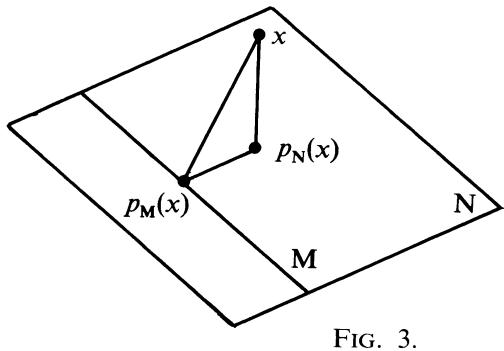
\includegraphics[keepaspectratio]{images/part002_dc4b20c6.jpg}}

